% Confirmation and controls: the strengthening campaign (.agent/notes/prereg_strengthen.md and its amendments).
% Owner: strengthening analyst. Final 2026-10-24: every block is complete and analysed. Every number is a macro
% from tables/num_strengthen.tex, written by paper/tables/strengthen_tables.py from
% .agent/notes/strengthen/analysis/<block>/ (scripts/strengthen_analysis.py and strengthen_diagnostic_report.py).
% An independent recomputation from the raw evaluator CSVs matches every contrast within 1e-14
% (.agent/notes/strengthen/verification/). Requires \InputIfFileExists{tables/num_strengthen}{}{} in
% the preamble. Main-text floats are input below; tables/float_strengthen_appendix.tex holds the appendix
% floats (see paper/INTEGRATION.md). Undefined numbers print a red ?? through \N.
\section{Confirmation and controls}\label{sec:confirm}

We registered four experiments and their tests before generating any of their images: a base-by-temperature factorial, a fixed temperature sweep, 150 fresh prompts and two more seeds per held-out prompt. Two development controls address the checkpoint and the flow shift. Intervals are nominal 95\% paired prompt-bootstrap intervals (2{,}000 draws); $^{*}$ marks a Holm-adjusted $p\le0.05$ within the registered family of each block. No setting was chosen from these results.

\begin{figure}[t]
\centering
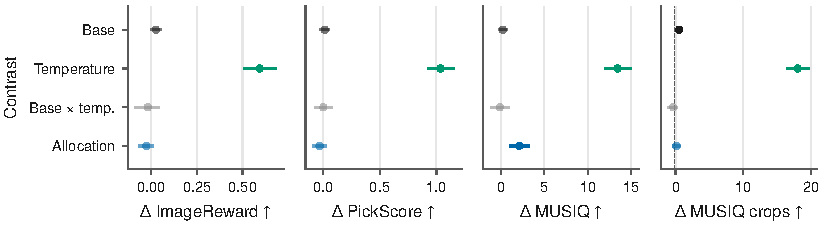
\includegraphics[width=\linewidth]{figs/strengthen/fs_factorial.pdf}
\caption{\textbf{The temperature carries the gain.} Paired contrasts on held-out rows 8 to 194 (seed 0, $n=\N{st@f@n}$): RoPE base and global temperature as main effects, their interaction, and the allocation (\segaofficial{} minus \tempsb). Whiskers are nominal 95\% intervals; marks are pale where the interval covers zero. \Cref{tab:strengthen-factorial-full} lists all ten metrics.}
\label{fig:fs-factorial}
\end{figure}

% Generated by paper/tables/strengthen_tables.py. Do not edit by hand.
\begin{table}[t]
\centering
\caption{\textbf{Factorial decomposition of \segaofficial.} Paired held-out contrasts on rows 8 to 194 ($n=187$ prompts, seed 0) from a 2$\times$2 design: RoPE base (\ntk{} or \sega) by global logit temperature (none or $s^{0.16}$), plus the allocation contrast (\segaofficial{} minus \tempsb). Main effects average the two levels of the other factor; the interaction is the temperature effect on the \sega{} base minus that on the \ntk{} base. Base, temperature and allocation add up to the whole gain of \segaofficial{} over \ntk{}. Cells give the paired mean difference with its nominal 95\% interval; triangles mark intervals that exclude zero, $^{*}$ marks Holm-adjusted $p\le0.05$ over the registered 80 tests (8 contrasts by 10 metrics), and bold marks the largest gain in each column. \Cref{tab:strengthen-factorial-full} expands this table to all eight contrasts and ten metrics. Key result: the global temperature improves all six displayed metrics under Holm (ImageReward $+0.594$, full-frame MUSIQ $+13.45$), neither the RoPE base nor the interaction survives Holm on any of the ten metrics, and the allocation improves full-frame MUSIQ ($+2.09$) while tying ImageReward and PickScore.}
\label{tab:strengthen-factorial}
\footnotesize
\setlength{\tabcolsep}{3.4pt}
% Generated by paper/tables/strengthen_tables.py. Do not edit by hand.
% Caption: \textbf{Factorial decomposition of \segaofficial.} Paired held-out contrasts (rows 8 to 194, $n=187$, seed 0) of a 2$\times$2 design, RoPE base (\ntk{} or \sega) by logit temperature (none or $s^{0.16}$), plus the allocation (\segaofficial{} minus \tempsb). Main effects average over the other factor; the interaction is the temperature effect on the \sega{} base minus that on the \ntk{} base. Base, temperature and allocation sum exactly to the total, \segaofficial{} minus \ntk, whose interval is computed directly; it is not a registered test. Cells give paired mean differences and nominal 95\% intervals; triangles mark intervals that exclude zero, $^{*}$ a Holm-adjusted $p\le0.05$ over the 80 registered tests, and bold the largest effect per column. \Cref{tab:strengthen-factorial-full} expands the table. Key result: the global temperature improves all six displayed metrics under Holm, neither the RoPE base nor the interaction survives Holm on any of the ten metrics, and the allocation improves full-frame MUSIQ ($+2.09$) while tying ImageReward and PickScore.
\begin{tabular}{@{}l rrrrrr@{}}
\toprule
Contrast & \makecell[r]{Image-\\Reward$\uparrow$} & \makecell[r]{Pick-\\Score$\uparrow$} & \makecell[r]{CLIP\\score$\uparrow$} & \makecell[r]{MUSIQ\\full$\uparrow$} & \makecell[r]{MUSIQ\\crop$\uparrow$} & \makecell[r]{CLIP-IQA\\full$\uparrow$} \\
\midrule
\multicolumn{7}{@{}l}{\emph{Main effects, averaged over the other factor}} \\
Base & \dcellT{+0.027}{-0.003}{+0.056} & \dcellT{+0.02}{-0.03}{+0.06} & \dcellT{-0.02}{-0.15}{+0.11} & \dcellT{+0.20}{-0.29}{+0.72} & \dcellB{+0.52}{+0.16}{+0.86} & \dcellT{+0.001}{-0.002}{+0.004} \\
Temperature & \dcellB{\mathbf{+0.594}^{*}}{+0.506}{+0.686} & \dcellB{\mathbf{+1.04}^{*}}{+0.92}{+1.16} & \dcellB{\mathbf{+2.03}^{*}}{+1.61}{+2.47} & \dcellB{\mathbf{+13.45}^{*}}{+11.96}{+15.11} & \dcellB{\mathbf{+18.07}^{*}}{+16.35}{+19.83} & \dcellB{\mathbf{+0.036}^{*}}{+0.021}{+0.050} \\
Base $\times$ temp. & \dcellT{-0.018}{-0.087}{+0.047} & \dcellT{+0.00}{-0.07}{+0.08} & \dcellB{+0.38}{+0.12}{+0.66} & \dcellT{-0.13}{-1.23}{+0.94} & \dcellT{-0.38}{-1.13}{+0.27} & \dcellT{-0.001}{-0.007}{+0.005} \\
\midrule
\multicolumn{7}{@{}l}{\emph{Per-band allocation}} \\
Allocation & \dcellT{-0.026}{-0.068}{+0.014} & \dcellT{-0.03}{-0.09}{+0.03} & \dcellT{-0.02}{-0.23}{+0.19} & \dcellB{+2.09^{*}}{+0.97}{+3.25} & \dcellT{+0.11}{-0.48}{+0.71} & \dcellB{+0.009}{+0.001}{+0.018} \\
\midrule
Total & \dcellB{+0.594}{+0.497}{+0.695} & \dcellB{+1.02}{+0.90}{+1.15} & \dcellB{+1.99}{+1.57}{+2.47} & \dcellB{+15.74}{+14.07}{+17.45} & \dcellB{+18.70}{+16.95}{+20.46} & \dcellB{+0.046}{+0.030}{+0.061} \\
\bottomrule
\end{tabular}

\end{table}


\paragraph{The temperature carries the gain, not the base}
\Cref{tab:strengthen-factorial} and \cref{fig:fs-factorial} complete the two-by-two design of RoPE base (\ntk{} or \sega) and global logit temperature (none or $s^{0.16}$) on the \N{st@f@n} held-out prompts. By construction, the two main effects and the allocation add up to the gain of \segaofficial{} over \ntk. Averaged over base, the temperature raises ImageReward by \N{st@f@d@temp@ir} \N{st@f@ci@temp@ir}, the whole \N{st@f@tot@ir} gain of \segaofficial{} over \ntk. It also raises full-frame MUSIQ by \N{st@f@d@temp@musiq} \N{st@f@ci@temp@musiq} of the \N{st@f@tot@musiq} total. Averaged over temperature, the \sega{} base changes ImageReward by \N{st@f@d@base@ir} \N{st@f@ci@base@ir} and full-frame MUSIQ by \N{st@f@d@base@musiq} \N{st@f@ci@base@musiq}. Its one nominal gain, \N{st@f@d@base@musiqc} \N{st@f@ci@base@musiqc} crop MUSIQ, does not survive Holm. The interaction survives Holm on no metric: the temperature raises ImageReward by \N{st@f@d@tempntk@ir} on the \ntk{} base and by \N{st@f@d@tempsega@ir} on the \sega{} base. Of the 80 registered tests, \N{st@f@nholm} survive Holm, \N{st@f@nholm@temp} for the temperature, \N{st@f@nholm@alloc} for the allocation, \N{st@f@nholm@base} for the base and \N{st@f@nholm@inter} for the interaction. \Cref{sec:decomp} credited base and temperature jointly; the factorial assigns that credit to the temperature.

\paragraph{The allocation moves image-quality scores, not rewards}
Within the same family, the allocation raises full-frame MUSIQ by \N{st@f@d@alloc@musiq} \N{st@f@ci@alloc@musiq} and crop CLIP-IQA by \N{st@f@d@alloc@iqac}. It also lowers the spectral slope error by \N{st@f@a@alloc@slope} and raises the tiling score by \N{st@f@a@alloc@tile}, a small loss, both surviving Holm. It ties ImageReward (\N{st@f@d@alloc@ir} \N{st@f@ci@alloc@ir}) and PickScore (\N{st@f@d@alloc@pick} \N{st@f@ci@alloc@pick}).

\paragraph{Reward and full-frame scores peak near $s^{0.16}$}
On the \sega{} base without allocation, five logit multipliers fixed before generation trace one curve on held-out rows 8 to 62 ($n=\N{st@s@n}$; \cref{tab:strengthen-sweep,fig:fs-sweep}). ImageReward is \N{st@sm@t100@ir} without temperature, \N{st@sm@t110@ir} at 1.1, \N{st@sm@tsref@ir} at $s^{0.16}$, \N{st@sm@tlogn@ir} at $\tau_N=4/3$ and \N{st@sm@t145@ir} at 1.45. No multiplier beats $s^{0.16}$ under Holm on ImageReward, PickScore or full-frame MUSIQ. Full-frame MUSIQ falls from \N{st@sm@tsref@musiq} at $s^{0.16}$ to \N{st@sm@t145@musiq} at 1.45, while crop MUSIQ rises at every step, from \N{st@sm@t100@musiqc} to \N{st@sm@t145@musiqc}. A crop-based quality score would therefore favour hotter attention than the reward models and the full-frame score do. \N{st@s@nholm} of the 40 sweep tests survive Holm.

\begin{figure}[t]
\centering
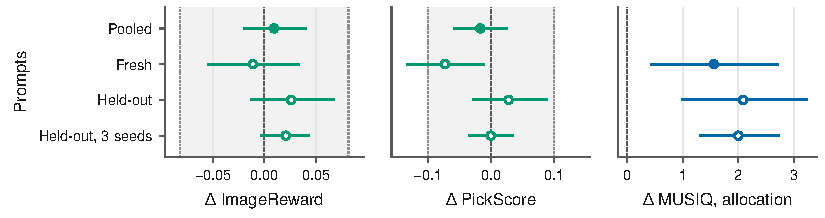
\includegraphics[width=\linewidth]{figs/strengthen/fs_confirm.pdf}
\caption{\textbf{Registered confirmation.} ImageReward and PickScore show \tempsb{} minus \segaofficial{} with the registered equivalence margins (gray band, dotted edges); full-frame MUSIQ shows the allocation (\segaofficial{} minus \tempsb). Filled marks are the registered tests (H1 on the pooled 337 prompts, H2 on the 150 fresh prompts); hollow marks are the fresh prompts alone, the held-out prompts at seed 0 and held-out prompt means over seeds 0 to 2.}
\label{fig:fs-confirm}
\end{figure}

% Generated by paper/tables/strengthen_tables.py. Do not edit by hand.
\begin{table}[!htbp]
\centering
\caption{\textbf{Registered confirmation.} $\Delta$ is \tempsb{} minus \segaofficial{} for H1 and the reverse for H2. H1 pools the 187 held-out prompts, inspected before registration, and 150 fresh prompts (seed 0) and needs both nominal intervals inside the margins and both Holm-adjusted equivalence $p\le0.05$; H2 uses the fresh prompts only and needs a positive lower bound and Holm $p\le0.05$. Holm runs over the three registered tests. The lower rows apply the same rules to the fresh prompts alone and to held-out prompt means over seeds 0 to 2, each with its own Holm family; they describe, but do not decide, the hypotheses. \Cref{tab:strengthen-fresh-arms,tab:strengthen-seeds} expand this table. Key result: H1 is supported on the pooled prompts and H2 is supported; on the fresh prompts alone the PickScore interval crosses the $-0.10$ margin, so equivalence is not established there.}
\label{tab:strengthen-fresh-tests}
\scriptsize
\setlength{\tabcolsep}{1.8pt}
% Generated by paper/tables/strengthen_tables.py. Do not edit by hand.
% Caption: \textbf{Registered confirmation.} $\Delta$ is \tempsb{} minus \segaofficial{} for H1 and the reverse for H2. H1 pools the 187 held-out and 150 fresh prompts (seed 0) and needs both nominal intervals inside the margins and both Holm-adjusted equivalence $p\le0.05$; H2 uses the fresh prompts only and needs a positive lower bound and Holm $p\le0.05$. Holm runs over the three registered tests. The lower rows apply the same rules to the fresh prompts alone and to held-out prompt means over seeds 0 to 2, each with its own Holm family; they describe, but do not decide, the hypotheses. Key result: H1 is supported on the pooled prompts and H2 is supported; on the fresh prompts alone the PickScore interval crosses the $-0.10$ margin, so equivalence is not established there.
\begin{tabular}{@{}l l r r r r l@{}}
\toprule
Test & Prompts & $\Delta$ & 95\% interval & Margin & Holm $p$ & Outcome \\
\midrule
\multicolumn{7}{@{}l}{\emph{Registered tests, one Holm family}} \\
H1 equivalence, ImageReward & 337 pooled & $+0.009$ & $[-0.020, +0.041]$ & $\pm0.082$ & $0.0015$ & \textbf{supported} \\
H1 equivalence, PickScore & 337 pooled & $-0.017$ & $[-0.059, +0.026]$ & $\pm0.100$ & $0.0015$ & \textbf{supported} \\
H2 superiority, full MUSIQ & 150 fresh & $+1.56$ & $[+0.43, +2.72]$ & $>0$ & $0.0045$ & \textbf{supported} \\
\midrule
\multicolumn{7}{@{}l}{\emph{Separately reported populations, same rules (descriptive)}} \\
H1 equivalence, ImageReward & 150 fresh & $-0.011$ & $[-0.055, +0.035]$ & $\pm0.082$ & $0.003$ & supported \\
H1 equivalence, PickScore & 150 fresh & $-0.073$ & $[-0.133, -0.011]$ & $\pm0.100$ & $0.2$ & not established \\
H1 equivalence, ImageReward & 187, 3 seeds & $+0.021$ & $[-0.004, +0.044]$ & $\pm0.082$ & $0.0015$ & supported \\
H1 equivalence, PickScore & 187, 3 seeds & $-0.000$ & $[-0.035, +0.037]$ & $\pm0.100$ & $0.0015$ & supported \\
H2 superiority, full MUSIQ & 187, 3 seeds & $+2.00$ & $[+1.30, +2.74]$ & $>0$ & $0.0015$ & supported \\
\bottomrule
\end{tabular}

\end{table}


\paragraph{Registered tests: equivalence and the MUSIQ gain hold}
H1 states that \tempsb{} is equivalent to \segaofficial{} on ImageReward (margin $\pm0.082$, half of \segaofficial's held-out gain over \dype) and on PickScore (margin $\pm0.10$). On the pooled 337 prompts the differences are \N{st@h@d@ir} \N{st@h@ci@ir} on ImageReward and \N{st@h@d@pick} \N{st@h@ci@pick} on PickScore, with Holm-adjusted equivalence $p=\N{st@h@p@ir}$ and $p=\N{st@h@p@pick}$. H2 states that the allocation raises full-frame MUSIQ on the 150 fresh prompts, where the difference is \N{st@h@d@musiq} \N{st@h@ci@musiq} (Holm $p=\N{st@h@p@musiq}$). The registered outcome is \emph{\N{st@h@H1}} for H1 and \emph{\N{st@h@H2}} for H2 (\cref{tab:strengthen-fresh-tests,fig:fs-confirm}). The pooled set reuses the 187 held-out prompts we had already inspected, so H1 extends the earlier tie rather than confirming it independently. On the fresh prompts alone, PickScore differs by \N{st@hf@d@pick} \N{st@hf@ci@pick}; this interval crosses the $-0.10$ margin, so fresh-only equivalence is \N{st@hf@status@pick}. ImageReward stays inside its margin there (\N{st@hf@d@ir} \N{st@hf@ci@ir}). We withdrew H3 before generation because its two controllers had already lost with tight intervals.

\paragraph{Fresh prompts reproduce the held-out ranking}
On the fresh prompts (\cref{tab:strengthen-fresh-arms}), ImageReward differs from \segaofficial{} by \N{st@e@d@ntk@ir} for \ntk, \N{st@e@d@segabase@ir} for the \sega{} base alone, \N{st@e@d@dype@ir} for \dype{} and \N{st@e@d@ntktemp@ir} \N{st@e@ci@ntktemp@ir} for \ntk{} with the temperature. As on the held-out set, \dype{} beats \segaofficial{} under Holm on crop MUSIQ (\N{st@e@d@dype@musiqc} \N{st@e@ci@dype@musiqc}) and CLIP-IQA (\N{st@e@d@dype@iqa}) while losing on ImageReward and PickScore (\N{st@e@d@dype@pick}). Both temperature arms trail \segaofficial{} on PickScore here, by \N{st@e@a@tsb@pick} on the \sega{} base and \N{st@e@a@ntktemp@pick} on the \ntk{} base. The held-out factorial showed no such gap, and the pooled H1 test averages over it. \N{st@e@nholm} of the 50 fresh secondary tests survive Holm.

\paragraph{Three seeds per prompt agree}
Averaging seeds 0, 1 and 2 within each held-out prompt ($n=187$ prompts, not 561 images), \tempsb{} minus \segaofficial{} is \N{st@rseeds012@d@tsb@ir} \N{st@rseeds012@ci@tsb@ir} on ImageReward, \N{st@hr@d@pick} \N{st@hr@ci@pick} on PickScore and \N{st@rseeds012@d@tsb@musiq} \N{st@rseeds012@ci@tsb@musiq} on full-frame MUSIQ (\cref{tab:strengthen-seeds}). Seeds 1 and 2 alone give \N{st@rseeds12@d@tsb@ir} \N{st@rseeds12@ci@tsb@ir} on ImageReward and \N{st@rseeds12@d@tsb@musiq} \N{st@rseeds12@ci@tsb@musiq} on full-frame MUSIQ. Each seed on its own also places the full-frame MUSIQ interval below zero.

\paragraph{The lattice is a checkpoint effect}
The dot lattice that led us to \krea{} could have come from guidance, since the earlier comparison ran \fluxdev{} at 3.5 and \krea{} at 4.5. With the official \dype{} code at matched guidance, \fluxdev{} carries \N{st@k@ratio@g3p5}$\times$ \N{st@k@ci@g3p5} the \krea{} lattice power at 3.5 and \N{st@k@ratio@g4p5}$\times$ \N{st@k@ci@g4p5} at 4.5 (8 development prompts, seed 42; \cref{tab:strengthen-ckpt}). On one bin chosen jointly for all four cells, raising guidance from 3.5 to 4.5 scales the \fluxdev{} lattice by \N{st@k@two@gdev}$\times$ \N{st@k@twoci@gdev} and the \krea{} lattice by \N{st@k@two@gkrea}$\times$ \N{st@k@twoci@gkrea}. Guidance modulates the lattice on \fluxdev, but the checkpoint gap remains at both values. \fluxdev{} also scores lower on ImageReward at both guidance values (\N{st@k@d@devminuskreag3p5@ir} at 3.5 and \N{st@k@d@devminuskreag4p5@ir} at 4.5). This is a descriptive development diagnostic.

\paragraph{The default flow shift degrades 4K samples}
The diffusers default extrapolates the flow shift to $\mu=11.55$ at $4096^2$, so the last model call sees $\sigma=\N{st@ds@sig@def}$; the official cap $\mu=1.15$ makes \N{st@ds@low@off} calls below $\sigma=0.3$ and ends at $\sigma=\N{st@ds@sig@off}$. On \N{st@ds@n} development prompts with \segaofficial{}, the default shift changes ImageReward by \N{st@ds@d@def@ir} \N{st@ds@ci@def@ir} and full-frame MUSIQ by \N{st@ds@d@def@musiq} \N{st@ds@ci@def@musiq}, and it worsens all ten metrics (\cref{tab:strengthen-default-shift}). Comparisons that mix the two schedules therefore confound the position embedding with sampling.

\paragraph{Second model family}
The registered Qwen-Image transfer test did not run. All 60 of its generation tasks failed with CUDA out-of-memory errors while a second process held about 45\,GiB of the same 95\,GiB GPU. A clean rerun did not fit the remaining compute budget. We therefore make no claim about other model families.
